\section{Data}

\begin{figure}[H]
    \centering
    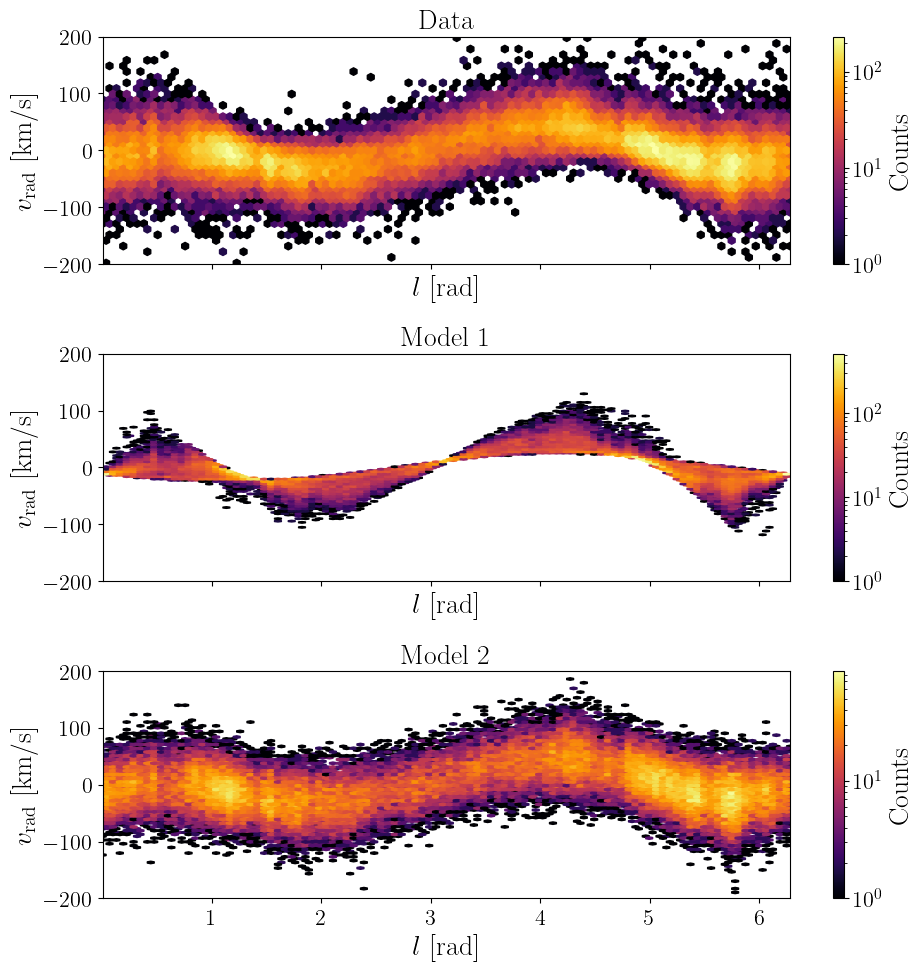
\includegraphics[width=0.95\columnwidth]{Fig/DataModelPresentation.png}
    \caption{Upper: radial velocities in the interval [-200, 200] \unit{\kilo\meter\per\second} of the used data. Middle: predictions of the radial velocities with the first model. Lower: simulation of the distribution of the radial velocities with the second model.}
    \label{fig:DataModelPresentation}
\end{figure}

In this work we use data collected by GAIA DR2~\cite{GAIADR2}. 
From the vast dataset of stars analyzed by GAIA, we select only those 
for which radial velocities, $v_{\text{rad}}$, were measured relative to the Sun using the Doppler effect. 
To manage the dataset size efficiently, we then apply a random selection to significantly reduce the quantity of data 
(imposing the random index of data to be less than 100000000).

For each selected star, we extract key parameters from GAIA DR2, 
including parallax $p$ and its associated error $\sigma_{\text{p}}$, 
radial velocity $v_{\text{rad}}$ with its measurement uncertainty $\sigma_{\text{v}}$, 
and galactic coordinates, i.e. latitude $b$ and longitude $l$.

To focus our analysis on stars located within the galactic plane, we impose a selection criterion of $\vert b \vert < 5^{\circ}$. 
Additionally, to ensure the reliability of the data, we retain only stars with a relative parallax error smaller than 20$\%$ 
and a radial velocity error below 5 \unit{\kilo\meter\per\second}. 
Following these criteria, 75659 stars were selected. The distribution of their radial velocity 
with respect to the Sun is plotted in the upper panel of figure \ref{fig:DataModelPresentation} 
as a function of their longitude. Only values in the interval 
[-200\unit{\kilo\meter\per\second}, 200\unit{\kilo\meter\per\second}] were reported for better visualisation. 
However, values up to 500 \unit{\kilo\meter\per\second} were observed. 
These are likely outliers, and a more sophisticated data selection procedure may improve the quality of the following analysis.
